\chapter{\label{ch:1-intro}Introduction} 

\graphicspath{{figures/ch1/}}

\minitoc

\section{Pancreatic islets and the \textgreek{b}-cell}

Pancreatic islets are endocrine cells which are responsible for maintaining glucose homeostasis.
It has been estimated that there are between \numrange{3e6}{1.5e7} islets in a human pancreas, constituting \SIrange{1}{2}{\percent} of the total pancreatic mass \cite{da_silva_xavier_cells_2018}.
Islets consist of three principal cell types; insulin secreting \textgreek{b}-cells, glucagon secreting \textgreek{a}-cells and somatostatin secreting \textgreek{d}-cells \cite{ashcroft_katp_2013}.
Islets respond to increases in blood glucose by releasing insulin, which acts on peripheral tissues to increase glucose uptake and reduce blood glucose levels.
Conversely, decreases in blood glucose leads to the release of glucagon, which acts on those tissues to stimulate glucose production and increase blood glucose.

Insulin secretion in beta cells - and indeed in all three cell types of pancreatic islets - is induced by the firing of action potentials, which leads to the influx of Ca\textsuperscript{2+} ions and the activation of secretory granule exocytosis (Figure \ref{ch1fig:beta_cells}) \cite{ashcroft_katp_2013}.
This electrical excitability is controlled by the ATP-sensitive potassium (K\ATP{}) channel.
At rest, K\ATP{} channel activity results in a leak current of K\textsuperscript{+} ions out of the cell, hyperpolarising the membrane.
Glucose metabolism in beta cells increases the ATP:ADP ratio, closing K\ATP{} channels and releasing their hyperpolarising clamp on the membrane potential \cite{ashcroft_glucose_1984-1, rorsman_glucose_1985-1}.
When K\ATP{} channels are closed and membrane resistance is high, even small currents are sufficient to induce large membrane potential depolarisations and action potential initiation (Figure \ref{ch1fig:beta_cells_firing}).

\begin{figure}[hbtp]
	\centering
	\begin{subfigure}[t]{0.9\textwidth}
		\caption{}\label{ch1fig:beta_cells}
		\centering
		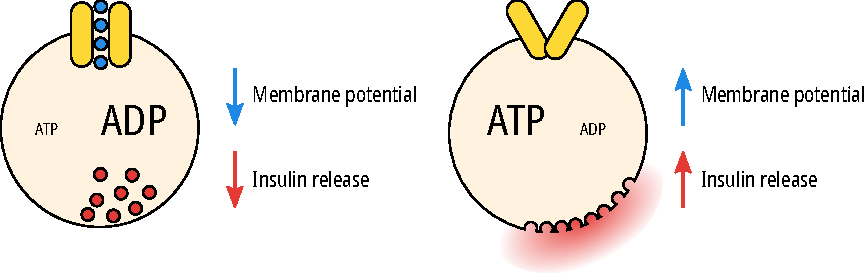
\includegraphics[width=\textwidth]{beta_cells.pdf}
	\end{subfigure}
	\vfill
	\begin{subfigure}[t]{0.9\textwidth}
		\caption{}\label{ch1fig:beta_cells_firing}
		\centering
		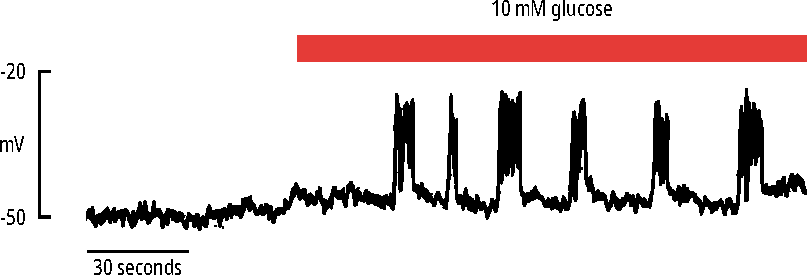
\includegraphics[width=\textwidth]{beta_cells_firing.pdf}
	\end{subfigure}
	\caption[Electrical excitability of pancreatic beta cells]{
		{\bf\mccorrect{Electrical excitability of pancreatic beta cells.}}
		\subref{ch1fig:beta_cells} When the ATP:ADP ratio is low, K\ATP{} channels are open, allowing K\textsuperscript{+} ions to flow out of the pancreatic beta cell and maintain a hyperpolarised membrane potential.
		When the ATP:ADP ratio is high, K\ATP{} channels close, allowing depolarisation of the membrane potential and insulin secretion.
		\subref{ch1fig:beta_cells_firing} Current record of a cell-attached patch of an isolated pancreatic beta cell, adapted from \textcite{rorsman_calcium_1986}. 
		Perfusion of glucose leads to depolarisation and action potential firing.
	}
	\label{ch1fig:beta_cells_overview}
\end{figure}

\section{Architecture of the pancreatic K\ATP{} channel}

K\ATP{} channels are present in many tissues, where they couple the metabolic state of a cell to its electrical activity by regulating the flow of K\textsuperscript{+} across the membrane \cite{nichols_k_2006}.
K\ATP{} channels are an octameric complex, comprised of four inwardly-rectifying potassium channel subunits (Kir6.1 or Kir6.2), each of which is associated with a sulphonylurea receptor subunit (SUR1, SUR2A or SUR2B) \cite{inagaki_family_1996, yamada_sulphonylurea_1997, shyng_octameric_1997, clement_association_1997}.
In pancreatic \textgreek{b}-cells, the K\ATP{} channel isoform is composed of Kir6.2 and SUR1 \cite{inagaki_reconstitution_1995}.
Together, Kir6.2 and SUR1 form a complex nearly a megadalton in size and over 15 nanometres across (Figure \ref{ch1fig:katp_cartoon}, \ref{ch1fig:sur_topdown}).

Inwardly-rectifying potassium channels are so named because they allow K\textsuperscript{+} to flow more easily into the cell than out of it (Figure \ref{ch1fig:rectification}) \cite{hille_ion_2001, zheng_handbook_2015}.
This phenomenon is a consequence of voltage-dependent pore blockade by intracellular divalent cations (especially Mg\textsuperscript{2+}) and polyamines.
At depolarising membrane potentials, blockers are driven into the pore and K\textsuperscript{+} current is blocked, while at hyperpolarising potentials the blockers and cleared and K\textsuperscript{+} current can flow.
Strongly rectifying Kir channels display drastically reduced conductance at potentials more positive than the K\textsuperscript{+} reversal potential.
In contrast, Kir6.2 is a weak rectifier, and allows substantial current to flow at more positive potentials.

In addition to voltage, Kir6.2 is regulated by two endogenous ligands; 
phosphatidylinositol 4,5-bisphosphate (PIP\textsubscript{2}) and adenine nucleotides (Figure \ref{ch1fig:kir_struct}) \cite{baukrowitz_pip2_1998, shyng_membrane_1998}.
The binding of adenine nucleotides to Kir6.2 leads to closure of the channel pore, while the binding of PIP\textsubscript{2} promotes the opening of the pore (Figure \ref{ch1fig:fan_trace}).
Activation by PIP\textsubscript{2} is a mechanism common to the whole Kir family, whereas inhibition by nucleotides is unique to the Kir6 subfamily \cite{enkvetchakul_direct_2005}.

\begin{figure}[hbtp]
	\centering
	\begin{subfigure}[t]{0.5\textwidth}
		\caption{}\label{ch1fig:rectification}
		\centering
		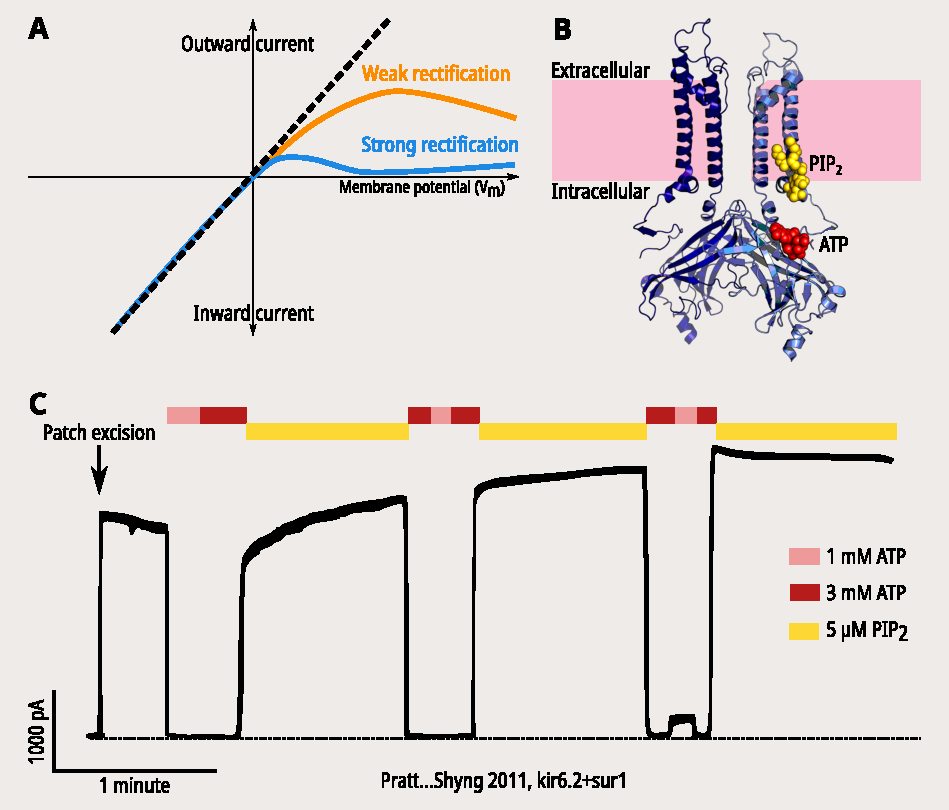
\includegraphics[width=\textwidth]{rectification.pdf}
	\end{subfigure}
	\hfill
	\begin{subfigure}[t]{0.4\textwidth}
		\caption{}\label{ch1fig:kir_struct}
		\centering
		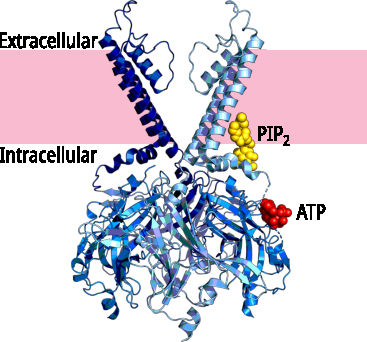
\includegraphics[width=\textwidth]{kir_structure.pdf}
	\end{subfigure}
	\vfill
	\begin{subfigure}[t]{0.6\textwidth}
		\caption{}\label{ch1fig:fan_trace}
		\centering
		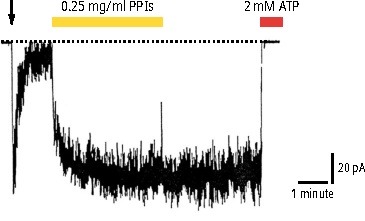
\includegraphics[width=\textwidth]{fan_pip_trace.pdf}
	\end{subfigure}
	\caption[Structure of Kir6.2]{
		{\bf\mccorrect{Structure of Kir6.2.}}
		\subref{ch1fig:rectification} Current-voltage plot demonstrating inward rectification of Kir channels.
		Here, the reversal potential of potassium (\textit{E\textsubscript{K}}) is set to zero, i.e. there is an equal concentration of K\textsuperscript{+} on each side of the membrane.
		Weak rectifiers such as Kir6.2 exhibit only a weak voltage dependent decline in conductance (visualised as a departure from the dashed line of an ideal conductor).
		(Adapted from \textcite{zheng_handbook_2015}).
		\subref{ch1fig:kir_struct} Cryo-EM structure of Kir6.2 (PDB \#6BAA) captured with ATP bound (red) and with the proposed binding position of PIP\textsubscript{2} visualised by alignment of the channel with the X-ray structure of Kir2.2 solved in compex with a short-chain dioctanoyl (diC8) PIP\textsubscript{2} (PDB \#6C3I).
		Unresolved residues in the structure are shown as dashed lines.
		The plasma membrane is shown in pink.
		(Adapted from \textcite{puljung_cryo-electron_2018}).
		\subref{ch1fig:fan_trace} Macroscopic currents from excised patches from pancreatic beta-cells clamped at \SI{-50}{\milli\volt}, adapted from \textcite{fan_anionic_1997}.
		Perfusion of ATP or phosphoinositides (PPIs) is indicated by coloured bars, and demonstrates the contrasting effects of these two ligands on channel activity.
		The zero current level is indicated by a dotted line.
		Patch excision is indicated with an arrow.
	}
	\label{ch1fig:kir_breakdown}
\end{figure}

SUR1 is a member of the ATP-binding cassette (ABC) family of transporters, \begin{mccorrection} first described by \textcite{higgins_family_1986}. \end{mccorrection}
While other ABC proteins transport substrate across the membrane, SUR1 does not appear to do so; instead it acts to modulate the function of its associated ion channel \cite{aguilar-bryan_cloning_1995, tusnady_membrane_1997}.
The cystic fibrosis transmembrane conductance regulator (CFTR) is another member of the ABC family, and is an ion channel in its own right, capable of conducting chloride across the membrane \cite{vergani_cftr_2005}.
Like other ABC proteins, SUR1 contains two sets of transmembrane domains (TMD1 and TMD2) and two cytosolic nucleotide binding domains (NBD1 and NBD2) \cite{aguilar-bryan_cloning_1995, ter_beek_structural_2014}.
Unique to SUR is the presence of an additional transmembrane domain (TMD0) N-terminal to the core of the protein, and this domain forms the primary contact between SUR1 and Kir6.2 \cite{lee_molecular_2017, martin_anti-diabetic_2017-1, li_structure_2017-1, martin_mechanism_2019-1}.

The NBDs of ABC transporters are highly conserved, and consist of two subdomains: a larger RecA-like subdomain found in other P-loop ATPases, and a smaller \textgreek{a}-helical subdomain which is unique to ABC transporters \cite{ter_beek_structural_2014, puljung_cryo-electron_2018}.
There are three key structural motifs present in these subdomains: the RecA-like subdomain contains the Walker A (W\textsubscript{A}) and B (W\textsubscript{B}) motifs, while the \textgreek{a}-helical subdomain contains the ABC signature motif (typically LSGGQ).

The two domains come together to form an antiparallel dimer with two nucleotide binding sites (NBS1 and NBS2) at the interface, such that NBS1 is formed from the W\textsubscript{A} and W\textsubscript{B} motifs of NBD1 and the signature motif from NBD2, whereas NBS2 is formed from the W\textsubscript{A} and W\textsubscript{B} motifs of NBD2 and the signature motif from NBD1.
NBS2, also known as the consensus site as it is more similar in sequence to other ABC family members, is catalytically competent and able to hydrolyse ATP \cite{matsuo_atp_1999, zingman_signaling_2001, de_wet_studies_2007}.
In contrast, NBS1 is the degenerate site, with a less conserved sequence and an inability to catalyse hydrolysis of ATP \cite{ter_beek_structural_2014, puljung_cryo-electron_2018}.

\begin{figure}[hbtp]
	\centering
	\begin{subfigure}[t]{0.4\textwidth}
		\caption{}\label{ch1fig:sur_struct}
		\centering
		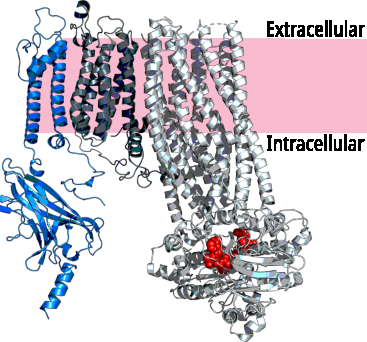
\includegraphics[width=\textwidth]{sur_structure.pdf}
	\end{subfigure}
	\hfill
	\begin{subfigure}[t]{0.5\textwidth}
		\caption{}\label{ch1fig:nbd_struct}
		\centering
		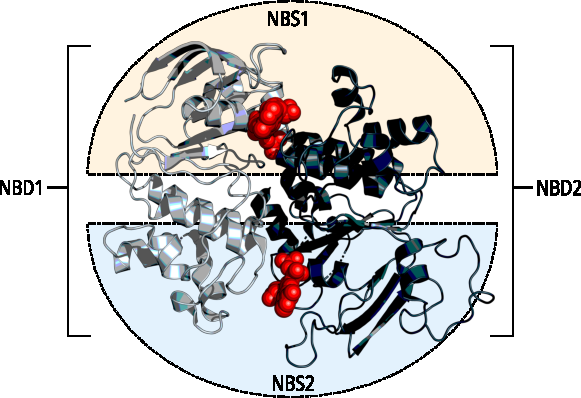
\includegraphics[width=\textwidth]{nbd_structure.pdf}
	\end{subfigure}
	\caption[Structure of SUR1]{
		{\bf\mccorrect{Structure of SUR1.}}
		\subref{ch1fig:sur_struct} Cryo-EM structure of SUR1 captured with a nucleotide (shown in red) bound at each NBS (PDB \#6C3P).
		A single SUR1 subunit is shown, with TMD1 and TMD2 in white and TMD0 in grey.
		A single Kir6.2 subunit is also shown in blue to show the interface between subunits.
		The plasma membrane is displayed in pink.
		\subref{ch1fig:nbd_struct} Top-down view of the NBDs from the same cryo-EM structure.
		NBD1 is on the left in silver, NBD2 is on the right in dark grey, and the two NBSs are higlighted; NBS1 in orange and NBS2 in blue.
		Adapted from \textcite{puljung_cryo-electron_2018}.
	}
\end{figure}

\section{Ligand-independent regulation of the pancreatic K\ATP{} channel}

\subsection{Assembly and trafficking}

Biogenesis of K\ATP{} channels occurs in the endoplasmic reticulum (ER), and is an important checkpoint in determining surface expression and channel stoichiometry \cite{zerangue_new_1999-1, martin_pharmacological_2013}.
The precise nature of the events which occur between subunit translation and insertion of octameric K\ATP{} into the cell membrane are not fully mapped out, but studies have highlighted some important quality control steps in this process which regulate K\ATP{} channel expression.
When Kir6.2 or SUR1 are expressed alone in heterologous systems, they are retained in the ER \cite{zerangue_new_1999-1}.
This mechanism is achieved through the exposure of a three amino acid ER-retention motif (RKR) in the cytoplasmic domains of both Kir6.2 and SUR1.
Only upon complete assembly of the channel complex are the RKR motifs masked, allowing forward trafficking of K\ATP{} to the cell surface.
Deletion of the RKR motif \cite{tucker_truncation_1997}, or mutation of the motif to AAA \cite{zerangue_new_1999-1}, results in unregulated surface expression of individual subunits and/or partially assembled channel complexes.
Addition of a GFP label to the C-terminus of Kir6.2 is also sufficient to allow trafficking of tetrameric Kir6.2 to the cell surface in the absence of SUR1 \cite{john_sulphonylurea_1998-1}.

In addition to the RKR motif, there are two N-linked glycosylation sites on SUR1 (N10 and N1050) which are required for cell surface expression \cite{conti_membrane_2002}.
Mutation of these sites to glutamines results in retention in the ER and drastically reduced expression of K\ATP{} on the cell surface.
This mechanism is thought to be separate to that for the ER-retention motif, as mutation of RKR to AAA is not sufficient to drive surface expression of the glycosylation mutants \cite{conti_membrane_2002}.

A putatitive third site of trafficking regulation is in the C-terminus of SUR1.
Mutation or deletion of a dileucine motif 16 amino acids distal to the C-terminal of SUR1 results in reduced surface expression of K\ATP{} channels in COSm6 cells \cite{sharma_c_1999}.
This reduction in expression is not rescued by C-terminal truncation of Kir6.2, indicating that this result is not due to masking of the RKR retention motif.
The dileucines are therefore suggested to promote forward trafficking of assembled channel complexes to the cell membrane \cite{sharma_c_1999}.
Expression of K\ATP{} channels expressed in \textit{Xenopus} oocytes is also dramatically reduced by truncation of the C-terminal 42 amino acids of SUR1 \cite{vedovato_role_2018}.
However, longer deletions of the SUR1 C-terminus did not reduce surface expression of channels in HEK293 cells \cite{giblin_cytoplasmic_2002}, and other modifications of the SUR1 C-terminus do not exhibit effects on surface expression \cite{schwappach_molecular_2000}.
In fact, a splice variant of SUR1 missing the entirety of the NBD2 domain (truncated at residue 1355) was found to successfully traffic to the cell membrane of \textit{Xenopus} oocytes \cite{sakura_altered_1999-1}.
The precise role of the dileucine motif remains unclear, and is potentially confounded by the use of expression system \cite{giblin_cytoplasmic_2002, martin_pharmacological_2013}

Failure of the channel complex to pass these three checkpoints results in ER-associated degradation (ERAD), a common pathway shared by most membrane and secretory proteins \cite{bonifacino_ubiquitin_1998, yan_role_2005}.
Both SUR1 and Kir6.2 are substrates for polyubiquitination, both when heterologously expressed and in INS-1 cells \cite{yan_role_2005}.
Application of proteasome inhibitors both reduces the rate of degradation for Kir6.2 and SUR1, and increases the surface expression of K\ATP{} channels by increasing their biogenesis efficiency \cite{yan_role_2005}.

The surface expression of K\ATP{} channels is therefore controlled by a variety of different quality control mechanisms to ensure that only correctly assembled octameric channel complexes reach the cell membrane.
Mutations which lead to defects in assembly and trafficking are therefore a common cause of congenital hyperinsulinemia (HI) as they result in permanent membrane depolarisation and unregulated insulin secretion.
These mutations are found throughout both Kir6.2 and SUR1, although they are more commonly found in SUR1 \cite{martin_pharmacological_2013}.

Interestingly, sulphonylureas are able to act as pharmacological chaperones and rescue surface expression of several mutations which would otherwise not traffic to the cell surface \cite{yan_sulfonylureas_2004, yan_sulfonylureas_2006, yan_congenital_2007, yan_congenital_2007-1, martin_pharmacological_2016}.
Sulphonylureas bind directly to the channel during biogenesis, as mutation of residues in SUR1 which are critical for sulphonylurea binding abolished or reduced the effectiveness of expression rescue \cite{yan_sulfonylureas_2006}.
Pharmacological chaperoning requires full assembly of the channel complex, as the presence of Kir6.2 was required to rescue expression of trafficking mutants even when the SUR1 RKR motif was mutated to AAA \cite{yan_sulfonylureas_2006}.
In addition, reducing the temperature at which cells are cultured can rescue some trafficking defects \cite{yang_low_2005}.

\begin{figure}[hbtp]
	\centering
	\begin{subfigure}[t]{0.9\textwidth}
		\caption{}\label{ch1fig:katp_cartoon}
		\centering
		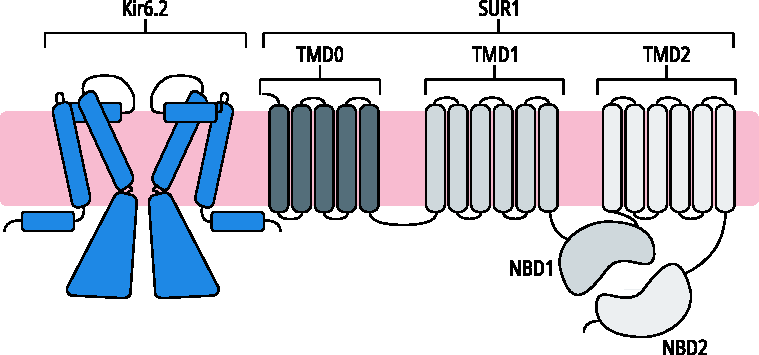
\includegraphics[width=\textwidth]{katp_cartoon.pdf}
	\end{subfigure}
	\vfill
	\begin{subfigure}[t]{0.45\textwidth}
		\caption{}\label{ch1fig:sur_topdown}
		\centering
		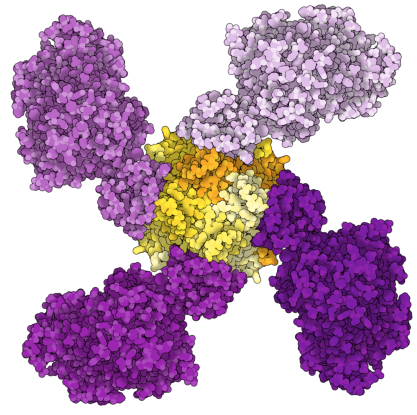
\includegraphics[width=\textwidth]{sur_topdown_propellor.pdf}
	\end{subfigure}
	\hfill
	\begin{subfigure}[t]{0.45\textwidth}
		\caption{}\label{ch1fig:sur_ctd}
		\centering
		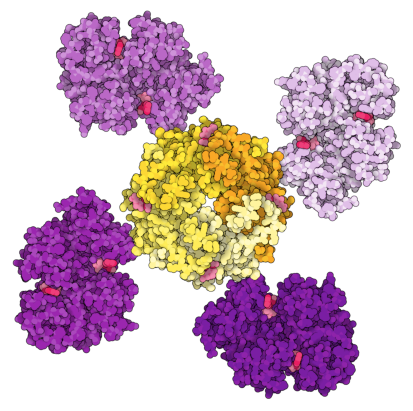
\includegraphics[width=\textwidth]{sur_topdown_ctd_propellor.pdf}
	\end{subfigure}
	\caption[K\ATP{} architecture and nucleotide regulation]{
		{\bf\mccorrect{K\ATP{} architecture and nucleotide regulation.}}
		\subref{ch1fig:katp_cartoon} Membrane topology of the K\ATP{} channel shown with two Kir6.2 subunits and one SUR1 subunit.
		\subref{ch1fig:sur_topdown} Top-down view of a cryo-EM structure of the K\ATP{} channel (PDB \# 6C3P) solved with nucleotides bound at each of the three canonical binding sites.
		Each SUR1 subunit is shown in a shade of purple, and each Kir6.2 subunit is shown in a shade of orange.
		\subref{ch1fig:sur_ctd} The same view of the structure shown to the left, but with the transmembrane domains removed to reveal the cytoplasmic domains of each subunit only.
		The nucleotides bound to the channel are shown in red.
	}
\end{figure}

\subsection{Regulation of intrinsic gating}

In the absence of nucleotides, K\ATP{} channels are spontaneously active.
This can be seen at a macroscopic level in excised patches.
Upon excision of a patch from a cell membrane containing K\ATP{} channels, the magnitude of current dramatically increases when voltage is applied (Figure \ref{ch1fig:fan_trace}), reflecting the relief from inhibition of cytoplasmic nucleotides.
While this macroscopic time course is smooth and graded, it consists of hundreds or thousands of individual channels which exhibit binary behaviour, switching between a nonconducting closed state and a conducting open state \cite{hille_ion_2001}.
The summed activity of these individual channels constitutes the large currents observed in macroscopic excised patches.

Single K\ATP{} channels exhibit bursts of brief openings, separated by long interburst closures \cite{alekseev_ligand-insensitive_1998, babenko_two_1999, li_open_2002, proks_modeling_2009}.
Thus, the open probability ($P_O$) of the channel is determined both by the kinetics of the burst (open and closed durations within a burst) and the duration of the long interburst closures.
The intrinsic gating of K\ATP{} can therefore be separated into two separate 'gating' processes; fast (responsible for intraburst closures) and slow (responsible for interburst closures).
While it is helpful to distinguish between fast and slow gating processes to characterise channel regulation, doing so does not require the existence of separate structural gates \cite{proks_modeling_2009, hille_ion_2001}.

Gating is a property intrinsic to Kir6.2, which is able to open and close in the absence of SUR1 \cite{tucker_truncation_1997, enkvetchakul_kinetic_2000-1} (Figure \ref{ch1fig:singles_sur}); albeit with very different kinetic properties as will be discussed later.
The open and intraburst closed time of single channels is dependent on the electrochemical gradient across the cell membrane, otherwise called the K\textsuperscript{+} driving force \cite{benz_characterization_1998}.
As the name implies, the electrochemical gradient depends on two things: the voltage across the membrane, and the K\textsuperscript{+} concentration gradient.
Increasing hyperpolarisation decreases the amount of time channels remain in the open state and increases the amount of time channels remain in the closed state within bursts \cite{alekseev_burst_1997, trapp_molecular_1998-1}.
This is a characteristic feature shared by other inwardly-rectifying K\textsuperscript{+} channels \cite{sakmann_voltage-dependent_1984, alekseev_burst_1997}.
In addition, altering the  K\textsuperscript{+} gradient across the membrane by changing the K\textsuperscript{+} concentration in the pipette or bath solution has the same effect on fast gating kinetics \cite{zilberter_gating_1988, benz_characterization_1998}.
As the driving force for K\textsuperscript{+} increases, the open lifetime of the K\ATP{} channel decreases.
This is in contrast to other K\textsuperscript{+} channels such as K\textsubscript{V}2.1, which exhibits the opposite relationship \cite{chapman_allosteric_2006}.

There are a number of domains within Kir6.2 that regulate the intrinsic gating of the channel.
Firstly, the P-loop is a conserved feature across K\textsuperscript{+} channels \cite{kuang_structure_2015}.
In Kir channels, the P-loop connects the two transmembrane domains, and dips into the plasma membrane to form the K\textsuperscript{+} selectivity filter.
While the P-loop is broadly conserved between Kir family members, there are key residues which differ.
Notably, the K\textsuperscript{+} selectivity filter signature sequence (TxGYG) is identical across all other Kir subtypes (TIGYG), but in Kir6.1 and Kir6.2 the tyrosine is replaced by a phenylalanine at position 133 (TIGFG), a feature shared by (\mccorrect{amongst others}) eag-like K\textsuperscript{+} channels \cite{heginbotham_mutations_1994}.
Another particularly interesting residue is V127, which is unique to Kir6.1 and Kir6.2 within the Kir family - all other Kir channels posess a threonine at this location \cite{proks_mutations_2001}.

\textcite{proks_mutations_2001} investigated a range of substitutions at these two residues.
Mutation of V127 to the conserved threonine (V127T) dramatically increases the open time of K\ATP{}, while also increasing the intraburst closed time.
There is also some suggestion of an additional open state existing in this mutant construct, evidenced by the appearance of a second peak in the open time histograms.
Mutation of F133 to the conserved tyrosine (F133Y) did not produce expression of functional channels; however combining the two mutations (V127T,F133Y) resulted in functional channels with a further increase in the open time when compared to the single mutant V127T.
In addition, substitutions at other residues in the P-loop of Kir6.2 lead to a range of effects on the intraburst kinetics of K\ATP{}.
Crucially, none of the substitutions affected the slow gating of the channel; i.e. burst duration and interburst closed times remained similar despite the varied alterations in the intraburst kinetics.
\textcite{proks_mutations_2001} concluded that the P-loop is instrumental in regulating the fast gating of K\ATP{}, and suggested that the lack of correlation between perturbations of inter- and intra-burst kinetics is evidence for independence between the fast and slow gating processes.

Other domains of Kir6.2 are involved in the regulation of slow gating.
The cytosolic end of the second transmembrane domain of Kir6.2 has been implicated in regulation of K\ATP{} slow gating by a number of mutational studies \cite{shyng_control_1997, tucker_molecular_1998, trapp_molecular_1998-1, loussouarn_structure_2000}.
Substitution of C166 with a more bulky or hydrophobic residue dramatically reduces the frequency of the channel entering the long, closed interburst state, and increases the open time of the channel in the bursts \cite{trapp_molecular_1998-1}.
However, no effect is seen on the length of the intraburst closed times, which is additional evidence for the independence of the fast and slow gating processes.
Substitutions at N160 \cite{shyng_control_1997}, L164 \cite{tammaro_kir62_2008}, I167 \cite{tucker_molecular_1998}, and T171 \cite{tucker_molecular_1998, drain_katp_1998} also increase channel open time and decrease the rate of entry into the interburst closed state, further implicating this region of Kir6.2 in modulating the slow gating of K\ATP{}.

The slide-helix of Kir6.2 is the interface between the transmembrane domain and the cytoplasmic domain, and mutations in this region result in changes in the single channel kinetics and $P_O$ of K\ATP{} \cite{proks_molecular_2004, koster_dend_2008, mannikko_interaction_2010, li_decomposition_2013,cooper_conserved_2017}.
Mutations examined at the single channel level show changes in burst duration \cite{proks_molecular_2004, koster_dend_2008, mannikko_interaction_2010} but unaltered intraburst kinetics.
Interpretation of the mechanism underlying these single channel kinetics alterations is complicated by the proximity of this region of Kir6.2 to the putative PIP\textsubscript{2} binding site \cite{pipatpolkai_evaluating_2020}.
Perturbations of this region could be affecting intrinsic gating directly, or indirectly by altering PIP\textsubscript{2} regulation, both of which would lead to changes in slow gating.

While Kir6.2 is able to gate intrinsically when expressed alone, coassembly with SUR1 alters the intrinsic gating of the channel in a number of ways.
Compared to the single channel kinetics of Kir6.2\textgreek{D}C or Kir6.2-GFP alone, coexpression of Kir6.2 with SUR1 increases the open time of the channel within the bursts, and increases their duration, while the intraburst closed times are unaffected \cite{trapp_molecular_1998-1, john_sulphonylurea_1998-1, chan_n-terminal_2003-1}.
This suggests that interactions of SUR1 with Kir6.2 serve to regulate the slow gating of the channel, rather than the fast gating.
The mechanisms by which SUR1 regulates intrinsic gating of the K\ATP{} channel are complex and not yet fully understood.
Structurally, the primary contacts between the two subunits are formed between the N-terminus and first transmembrane domain of Kir6.2 and TMD0 and L0 of SUR1 (Figure \ref{ch1fig:sur_struct}) \cite{martin_anti-diabetic_2017, lee_molecular_2017-1, li_structure_2017-1}.
The contributions of the interactions of these regions have been studied in a variety of ways.

\begin{figure}[hbtp]
	\centering
	\begin{subfigure}[t]{0.45\textwidth}
		\caption{}\label{ch1fig:singles_ploop}
		\centering
		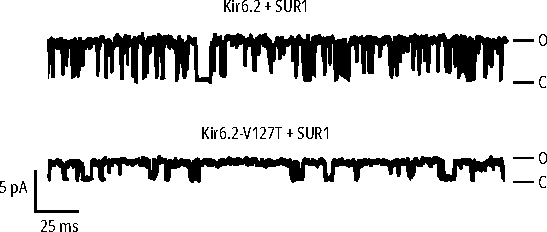
\includegraphics[width=\textwidth]{single_traces_ploop.pdf}
	\end{subfigure}
	\hfill
	\begin{subfigure}[t]{0.45\textwidth}
		\caption{}\label{ch1fig:singles_sur}
		\centering
		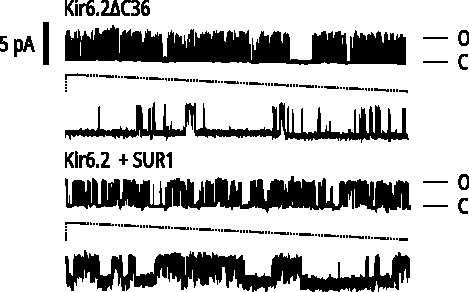
\includegraphics[width=\textwidth]{single_traces_sur.pdf}
	\end{subfigure}
	\vfill
	\begin{subfigure}[t]{0.45\textwidth}
		\caption{}\label{ch1fig:sur_shift}
		\centering
		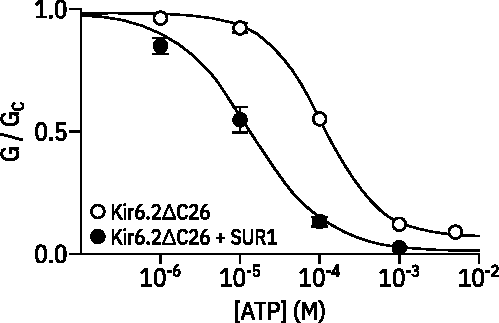
\includegraphics[width=\textwidth]{tucker_sur_shift.pdf}
	\end{subfigure}
	\hfill
	\begin{subfigure}[t]{0.45\textwidth}
		\caption{}\label{ch1fig:intrinsic_diagram}
		\centering
		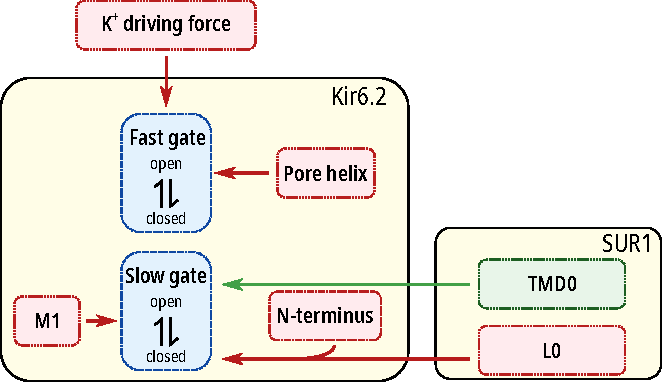
\includegraphics[width=\textwidth]{regulation_diagram_2.pdf}
	\end{subfigure}
	\caption[Intrinsic regulation of Kir6.2 gating]{
		{\bf\mccorrect{Intrinsic regulation of Kir6.2 gating.}}
		\subref{ch1fig:singles_ploop} Single channel recordings of excised patches from oocytes either expressing SUR1 with either Kir6.2 or Kir6.2-V127T in symmetrical 140 mM K\textsuperscript{+} at a membrane potential of -60 mV.
		Adapted from \textcite{proks_mutations_2001}.
		\subref{ch1fig:singles_sur} Single channel recordings of excised patches from cultured cells either expressing Kir6.2 alone with the C-terminal 36 amino acids truncated (Kir6.2\textgreek{D}C36) or coexpressing wild-type Kir6.2 with SUR1 in symmetrical 140 mM K\textsuperscript{+} at a membrane potential of \SI{-50}{\milli\volt}.
		Adapted from \textcite{enkvetchakul_kinetic_2000-1}.
		In both panels, openings leading to inward currents are displayed as upward deflections.
		Note that the timescales differ slightly between panels as traces are from two separate papers.
		\subref{ch1fig:sur_shift} Concentration-response relationship of ATP from macroscopic currents excised from \textit{Xenopus} oocytes injected with either Kir6.2\textgreek{D}C26 mRNA alone (open circles), or a mixture of Kir6.2\textgreek{D}C26 and SUR1 mRNAs (closed circles).
		Response is given as the fraction of the slope conductance (G) remaining during exposure to ATP.
		Adapted from \textcite{tucker_truncation_1997}.
		\subref{ch1fig:intrinsic_diagram} The intrinsic open-closed equilibrium of the pancreatic K\ATP{} channel pore is regulated by the K\textsuperscript{+} driving force and by the presence of different SUR1 domains.
	}
\end{figure}

\textcite{babenko_two_1999} constructed a series of SUR1/SUR2A chimeras and characterised the changes in single channel kinetics that resulted from swapping different domains between the two isoforms of SUR.
They found that Kir6.2+SUR2A channels exhibited a far higher single channel $P_O$ than Kir6.2+SUR1 channels (0.91 and 0.64 respectively).
This difference could be attributed to increased burst durations and decreased interburst periods, while fast gating was indistinguishable.
They found that a chimerical construct replacing the N-terminal 291 amino acids of SUR1 with those of SUR2A was sufficient to recapitulate the single channel kinetics of full-length SUR2A, suggesting that this region is critical for specifying the intrinsic gating of K\ATP{}.

Later work established that truncations of SUR1 to TMD0 or TMD0-L0 fragments allowed expression of "mini-K\ATP{}" channels at the cell membrane \cite{babenko_sur_2003, chan_n-terminal_2003, fang_n-terminal_2006}.
The first two studies showed that expression of Kir6.2 with TMD0 alone (residues 1-195 or 1-196 of SUR1) essentially recapitulates the intrinsic gating characteristics of Kir6.2 expressed with full-length SUR1, restoring the increased open time duration and burst duration as compared to expression of Kir6.2 alone \cite{babenko_sur_2003, chan_n-terminal_2003}.
\textcite{fang_n-terminal_2006} later found that in their hands, mini-K\ATP{} channels formed from Kir6.2\textgreek{D}C and SUR1-TMD0 were similar to full-length K\ATP{} but they consistently observed differences in the burst durations.
This discrepancy may be, at least in part, due to differences in the heterologous expression system (COSm6 cells in \textcite{babenko_sur_2003}, \textit{Xenopus} oocytes in \textcite{fang_n-terminal_2006}).
Otherwise, the remaining difference between K\ATP{} and mini-K\ATP{} channels could either be due to differences in structural interactions due to the truncation, or could implicate a role for the ABC core domain in regulating slow gating \cite{fang_n-terminal_2006}.

Increasing the length of the SUR1 fragment to include the first section of the L0 linker (residues 1-232 of SUR1) results in a nearly constitutively open channel, with dramatically increased open time duration and few observable interburst closures \cite{babenko_sur_2003}.
The resulting $P_O$ of 0.93 reflects a near saturation of the slow gating process; as without changes to the fast gating there can be limited further increases in $P_O$ due to the flickery closure.
Increasing the length of the L0 linker included in the SUR1 truncation fragment results in a progressive decrease in the open time duration, burst length and $P_O$, although it never regresses to the kinetics observed in Kir6.2 expressed alone \cite{babenko_sur_2003}.
These findings suggest that while the TMD0 and the initial segment of L0 help to stabilise the open state of K\ATP{} channels, other sections of the L0 linker act to destabilise the open state in some fashion \cite{babenko_sur_2003, puljung_cryo-electron_2018-1}.

One hypothesis for this destabilisation is that parts of the L0 linker interact with the N-terminus of Kir6.2 to regulate the intrinsic gating of K\ATP{} channels \cite{koster_atp_1999, babenko_n-terminus_1999, reimann_involvement_1999-1, babenko_sur-dependent_2002}.
When Kir6.2\textgreek{D}C is expressed alone, deletion of the first 14 amino acids of the N-terminus of Kir6.2 does not affect the single channel kinetics \cite{reimann_involvement_1999-1}.
However, in the presence of SUR1, truncations of up to the first 44 amino acids of the N-terminus reduce the frequency of transitions to the long closed state, increasing the $P_O$ \cite{reimann_involvement_1999-1, koster_atp_1999, babenko_n-terminus_1999}.
This effect increases with progressive truncations from \textgreek{D}N4 to \textgreek{D}N30, but increasing the truncation past this point does not appear to have additional effects.

\textcite{cukras_role_2002} conducted an alanine scan of positively charged residues in the N-terminus of Kir6.2.
They identified two residues in the proximal 30 amino acids which reduced $P_O$ when substituted (R4A, K5A) and two residues which increased $P_O$ when substituted (R16A, R27A).

Application of a synthetic peptide which contains the first 33 amino acids of the N-terminus of Kir6.2 to full-length K\ATP{} channels decreases the frequency of transitions to the closed state, in a manner comparable to truncation of the N-terminus \cite{babenko_sur-dependent_2002}.
This effect was dependent on the presence of SUR1, as with the N-terminal truncation experiments.
This finding suggests that the synthetic peptide competes with the endogenous N-terminus of Kir6.2 for an interaction within the K\ATP{} channel complex.

Finally, \textcite{craig_-frame_2009} investigated an in-frame deletion of five amino acids (28\textgreek{D}32) identified in neonatal diabetes patients.
This deletion resulted in K\ATP{} channels with increased $P_O$ only in the presence of SUR1; single Kir6.2\textgreek{D}C and Kir6.228\textgreek{D}32,\textgreek{D}C channel currents were indistinguishable.
The authors then made use of the 1-195 and 1-288 truncated SUR1 constructs described by \textcite{babenko_sur_2003}, and determined that only when the L0 linker was present (i.e. SUR1 residues 1-288) was there a difference in intrinsic gating upon the 28\textgreek{D}32 deletion.

Together, these results provide evidence for interactions between SUR1 and the N-terminus of Kir6.2 which facilitate transitions to the long closed state of the channel \cite{babenko_sur_2003}.

Of course, when measuring currents from hundreds or thousands of K\ATP{} channels, it is not possible to distinguish between perturbations which alter fast gating and perturbations which alter slow gating; the current measured reflects the sum of both of these processes.
At a macroscopic level, anything which increases single channel open time or burst duration, or decreases the intraburst closed time or frequency of entering the interburst state will be indistinguishable.

\section{Ligand dependent regulation of the pancreatic K\ATP{} channel}

K\ATP{} channels are regulated by two classes of endogenous ligands (nucleotides and phosphoinositides) and a range of exogenous ligands (predominantly sulphonylureas and glinides) (Figure \ref{ch1fig:regulation_diagram}).
Thus far, the action of each of these ligands appears to exclusively affect the slow gating of channel \cite{proks_modeling_2009}.
While the binding of adenine nucleotides to the Kir6.2 binding site leads to closure of the pore, binding of nucleotides to the NBSs of SUR1 in the presence of Mg\textsuperscript{2+} activates the channel \cite{nichols_adenosine_1996-1, vedovato_nucleotide-binding_2015}.
The interplay between the action of nucleotides at these distinct sites (Figure \ref{ch1fig:sur_ctd}) determines the response of the K\ATP{} channel to metabolic changes, and therefore even subtle mutations or modifications to these sites can lead to diseases of insulin secretion.
Phosphoinositides present in cell membranes are also regulators of K\ATP{} function, a property which is shared amongst the Kir family of channels \cite{fan_anionic_1997, nichols_k_2006, hibino_inwardly_2010}.
PIP\textsubscript{2} stimulates the opening of K\ATP{}, and excision of membrane patches results in a decline of channel activity due to the loss of PIP\textsubscript{2} in the excised membrane over time \cite{proks_running_2016-2}.

Proteins are inherently dynamic and sample a vast ensemble of accessible conformations \cite{boehr_role_2009}.
Techniques with high temporal resolution such as NMR spectroscopy have revealed the breadth of the energy landscape of macromolecules, and highlighted the ability of molecules at equilibrium to adopt a variety of conformational states \cite{mittermaier_new_2006}.
The K\ATP{} channel is no exception.
The ability of the channel to open and close in the absence of ligand (i.e. after channel rundown due to loss of PIP\textsubscript{2}) shows that at equilbrium, the K\ATP{} channel is able to exchange between open and closed states, albeit with a much higher occupancy of closed states \cite{ribalet_regulation_2000, proks_running_2016-2}.
One mechanism by which ligands are proposed to regulate the equilibrium of K\ATP{} channels (and macromolecules in general) is by being selective for particular conformations.
For example, PIP\textsubscript{2} will exhibit a higher binding affinity for the open state of the channel that it will for the closed state; and thus the presence of PIP\textsubscript{2} will selectively stabilise the open state of K\ATP{} channels.
This mechanism is the cornerstone of the MWC model of allostery \cite{monod_nature_1965-1, rubin_nature_1966, garcia_chapter_2011, marzen_statistical_2013}, and its assumptions and implications will be discussed in more detail in \ref{ch:4}.
In this framework, the link between ligand binding and channel gating, sometimes called transduction, is the factor by which a ligand preferentially stabilises a particular conformation.
Figure \ref{ch1fig:regulation_diagram} is a simplified diagram of how ligands interact to regulate the K\ATP{} channel.
Briefly, $L$ describes the unliganded equilibrium between open and closed states, while ligands which bind with affinity constants $K_X$ preferentially stabilise the open state by a factor $D_X > 1$ or the closed state by a factor $D_X < 1$ (where $X$ is the general term for a particular ligand interaction).

\begin{figure}[hbtp]
	\centering
	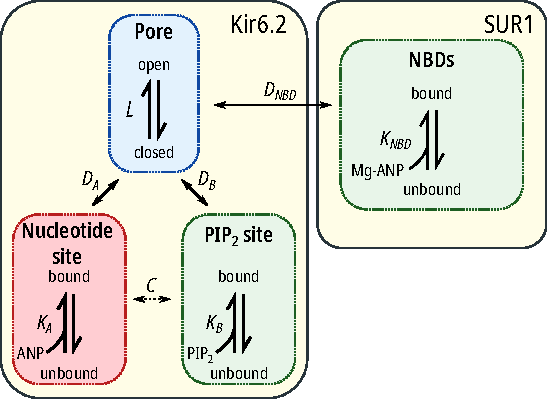
\includegraphics[width=0.7\textwidth]{regulation_diagram.pdf}
	\caption[Modes of regulation of K\ATP{}]{
	{\bf\mccorrect{Modes of regulation of K\ATP{}.}}
	Adapted from \textcite{puljung_cryo-electron_2018}.
	The open-closed equilibrium of the K\ATP{} channel pore (denoted as $L$) is energetically coupled to three different ligand binding sites.
	The four inhibitory nucleotide binding sites of Kir6.2 bind either ATP or ADP (generalised to ANP) with an equilbrium binding constant $K_A$.
	The four stimulatory PIP\textsubscript{2} binding sites of Kir6.2 bind PIP\textsubscript{2} with an equilbrium binding constant $K_B$.
	The four stimulatory Mg-nucleotide binding sites formed by the dimerisation of the NBDs of SUR1 (labelled as NBDs) bind either ATP or ADP with an equilbrium binding constant $K_C$, and Mg\textsuperscript{2+} is required for transduction.
	Each binding domain interacts with the channel pore according to the factors $D_A$, $D_B$, and $D_{NBD}$ respectively.
	In addition, there is a potential coupling between the inhibitory nucleotide binding site of Kir6.2 and the stimulatory PIP\textsubscript{2} binding site of Kir6.2 described by the factor $C$.
	}\label{ch1fig:regulation_diagram}
\end{figure}

\subsection{Nucleotide regulation of the pancreatic K\ATP{} channel}

The physiological regulation of channel activity by nucleotides is the summed contribution of activation by Mg-nucleotides binding to the NBSs of SUR1, and inhibition by nucleotides binding to Kir6.2 \cite{nichols_adenosine_1996}.
To study these contributions experimentally, most research to date has relied on electrophysiological recordings of K\ATP{} currents.
Separating the contributions of the different classes of site has been achieved through a variety of methods.
Firstly, activation of the channel by Mg-nucleotides can be eliminated by removing Mg\textsuperscript{2+} ions from the solutions used to perfuse excised patches by inclusion of high concentrations of chelators such as EDTA or EGTA \cite{gribble_mgatp_1998-1, proks_activation_2010-1}.
While it may still be possible that nucleotides bind to the NBDs in the absence of Mg\textsuperscript{2+} ions and affect channel inhibition, it is widely assumed that the absence of Mg\textsuperscript{2+} ions allows for the measurement of inhibition at Kir6.2 alone. 
Secondly, activation of the channel by Mg-nucleotides can be isolated by introducing mutations which abolish nucleotide binding to Kir6.2 \cite{gribble_mgatp_1998-1, proks_activation_2010-1}.

Mutation of residues which are involved in nucleotide inhibition of the K\ATP{} channel can result in one of two functional effects.
In the first category are residues which, when substituted, reduce the sensitivity of the channel to nucleotide inhibition (i.e. increase the IC\textsubscript{50} for nucleotide inhibition) while not perturbing the intrinsic gating of the channel.
Mapping these residues to the cryo-EM structures of ATP-bound K\ATP{} channels reveals that the residues in this category are invariably located close to the nucleotide binding site of Kir6.2.
The binding site is composed of part of the N-terminal region of one Kir6.2 subunit, and part of the C-terminal region of its neighbouring subunit.
Well characterised mutations of residues in this region of the N-terminus (e.g. R50 \cite{proks_involvement_1999, cukras_role_2002, john_molecular_2003, ribalet_molecular_2003, trapp_identification_2003, shimomura_mutations_2006}, and G53 \cite{koster_dend_2008}) and the C-terminus (e.g. I182 \cite{drain_katp_1998, koster_atp_2005, li_i182_2000}, K185 \cite{john_molecular_2003, ribalet_molecular_2003, trapp_identification_2003}, F333 \cite{tammaro_kir62_2005}, and G334 \cite{drain_katp_1998, tammaro_kir62_2005, masia_atp-binding_2007-1, proks_activation_2010-1}) have no effect on the single channel kinetics in the absence of nucleotide.
However, they are far less sensitive to inhibition by nucleotides.
The simplest hypothesis to explain this data given the location of the residues in the structures is that mutations of these residues perturb interactions between K\ATP{} and nucleotides, reducing the direct binding affinity of nucleotides for the inhibitory binding site (i.e. a reduction of $K_A$ in Figure \ref{ch1fig:regulation_diagram}).

Alternatively, mutations which do not affect intrinsic gating but reduce sensitivity to nucleotide inhibition may be decreasing the efficacy of nucleotides, rather than the affinity, causing nucleotide binding to no longer be as strongly coupled to the pore (i.e. $D_A$ approaches unity in Figure \ref{ch1fig:regulation_diagram}).
R201 was hypothesised to form part of the binding site as a cysteine \cite{proks_molecular_2004, antcliff_functional_2005} or histidine \cite{tammaro_functional_2006} substitution at this site results in reduced inhibition of K\ATP{} channels by nucleotides, without any changes in intrinsic gating .
Curiously, an alanine at this position results in K\ATP{} channels which exhibit both reduced sensitivity to ATP inhibition and reduced activation by PIP\textsubscript{2} \cite{shyng_structural_2000}.
Examining the cryo-EM structures suggests that this residue does not form direct contacts with bound ATP, and would therefore have to alter the nucleotide binding site allosterically - potentially by stabilising the short helix containing the critical F333 and G334 residues \cite{puljung_cryo-electron_2018}.
\textcite{ribalet_molecular_2003, john_molecular_2003} proposed that mutating R201 to an alanine instead acts by perturbing the preference of nucleotides for the closed state of the channel, increasing $D_A$.

The second category of residues are those which, when mutated, increase the $P_O$ of the channel and also affect the sensitivity of the channel to nucleotide inhibition.
This category is far larger, and these residues are found across both Kir6.2 and SUR1 structures.
Within the MWC framework in Figure \ref{ch1fig:regulation_diagram}, mutations which increase $L$ (and therefore increase the observed $P_O$) reduce the ability of nucleotides to inhibit the channel.
By increasing the stability of the open state, the selectivity of nucleotides for the closed state ($D_A < 1$) results in a decreased probability of nucleotide binding, and thus reduces inhibition.
Mutations within this category are difficult to fully characterise in the cell membrane environment due to the presence of phosphoinositides.
An observed increase in $P_O$ in an excised patch may either stem from an increase in $L$, or from an increase in $K_B$ or $D_B$.

Activation of K\ATP{} channels by Mg-nucleotides is not quite as trivial to measure in isolation.
The most common experimental paradigm used to isolate stimulatory effects is introduction of a mutation into Kir6.2 which renders it insensitive to inhibition by nucleotides \cite{gribble_mgatp_1998-1, proks_activation_2010-1}.
Application of Mg-nucleotides to mutant channels such as Kir6.2-G334D then results in an increase in the burst duration and therefore the $P_O$ of K\ATP{} channels \cite{proks_activation_2010-1}.
This stimulatory effect is conferred by the NBSs of SUR1, as mutation of the Walker A motif in either NBS1 or NBS2 results in K\ATP{} channels which are no longer activated by Mg-nucleotides \cite{gribble_essential_1997,nichols_adenosine_1996}.

In ABC transporters, the conformational changes which allow substrate movement across the membrane are driven by ATP hydrolysis \cite{rees_abc_2009}.
In addition, there is strict coupling between ATP hydrolysis and channel gating in CFTR, an ABC family member which is in itself a chloride channel \cite{csanady_strict_2010-1}.
The NBDs of SUR are capable of hydrolysing ATP at rates comparable to that of CFTR \cite{matsuo_atp_1999, wet_studies_2007, puljung_cryo-electron_2018}, although by necessity these studies were carried out on purified channels or purified NBD fragments and may not reflect the physiological rate.
\textcite{zingman_signaling_2001-1} used beryllium-fluoride and orthovanadate to stabilise the pre- and post-hydrolytic states of SUR2A respectively, and suggested that the post-hydrolytic state favoured channel opening.

However, \textcite{choi_testing_2008} analysed the microscopic reversibility of single-channel kinetics to determine whether ATP hydrolysis is coupled to channel gating.
Microscopic reversibility is a property of equilibrium systems such that their dynamics are time-reversible.
As ATP hydrolysis is irreversible and thus not in equilibrium, if channel gating is dependent on ATP hydrolysis it will not obey microscopic reversibility \cite{rothberg_testing_2001}.
Unlike for CFTR \cite{csanady_strict_2010-1}, \textcite{choi_testing_2008} found no evidence for ATP-dependent violations of microscopic reversibility in K\ATP{} channel gating, supporting the conclusion that ATP hydrolysis by the NBDs of SUR1 is not directly coupled to conformational changes of the channel.
In addition, Mg-ADP is sufficient to activate channel currents, obviating the need for ATP hydrolysis \cite{proks_activation_2010-1}.
It is most likely that the activatory function of Mg-nucleotides occurs in a similar manner as for the inhibitory function of nucleotides; via an allosteric equilibrium effect on the channel pore ($D_{NBD}$ in Figure \ref{ch1fig:regulation_diagram}).
It remains unclear whether Mg-ATP is capable of activating K\ATP{} channel currents upon binding to SUR1, or whether it first needs to be hydrolysed to Mg-ADP.

\subsection{PIP\textsubscript{2} regulation of the pancreatic K\ATP{} channel}

A conserved feature of Kir channels is that they are regulated by phosphoinositides, in particular PIP\textsubscript{2}, and Kir6.2 is no exception \cite{hibino_inwardly_2010, fan_anionic_1997, shyng_membrane_1998, baukrowitz_pip2_1998}.
Studying the nature of the regulation of K\ATP{} by PIP\textsubscript{2} is difficult experimentally due to the lack of control over PIP\textsubscript{2} concentrations, and our inability to precisely measure them.
Firstly, while the contaminating effects of intracellular nucleotides are removed by excision of a patch, the same is not true for PIP\textsubscript{2}.
The rundown of channel currents is largely attributable to dissociation and/or degradation of PIP\textsubscript{2} from the membrane patch, but rundown is a complex phenomenon and the relative amounts of PIP\textsubscript{2} in the membrane varies between patches and experimental conditions \cite{proks_running_2016-2}.
The hydrophobicity of PIP\textsubscript{2} means that perfusing a membrane patch with it results in accumulation of lipid in the membrane; it is impossible to reach an equilibrium with a known concentration.
An alternative is using analogs of PIP\textsubscript{2} with increased solubility due to shortening of the acyl chain length, such as dioctanoyl (diC\textsubscript{8}) PIP\textsubscript{2} \cite{rohacs_specificity_2003}.
While more soluble analogs are easier to work with and an experimenter can reach a quasi-equilibrium, we still do not know how the concentration of diC\textsubscript{8} PIP\textsubscript{2} applied to the membrane equates to the concentration achieved in the membrane; nor do we know if soluble analogs such as diC\textsubscript{8} PIP\textsubscript{2} modulate the channel in exactly the same manner as PIP\textsubscript{2}.
Another alternative is using polyamines such as neomycin as negative charge chelators; screening the negatively-charged phospholipid head groups present in the membrane away from their normal binding sites \cite{fan_anionic_1997, schulze_phosphatidylinositol_2003}.
This approach runs into the problems of both methods previously outlined; we do not know the precise correlation between the concentration of neomycin applied and the concentration of active, un-chelated PIP\textsubscript{2} in the membrane; and due to rundown it is impossible to reach a true equilibrium.
It also remains possible that neomycin may have additional effects independent of PIP\textsubscript{2} screening.

Despite all these complexities, there is still a great deal of research exploring how PIP\textsubscript{2} regulates K\ATP{} channel gating.
Many researchers have shown that PIP\textsubscript{2} stimulates K\ATP{} channel currents by increasing channel open time and burst duration, and reduces the sensitivity of K\ATP{} channel currents to inhibition by nucleotides \cite{fan_phosphoinositides_1999, baukrowitz_pip2_1998, shyng_membrane_1998, fan_phosphoinositides_1999, enkvetchakul_kinetic_2000}.
The stimulatory effect occurs in the absence of SUR1, as the $P_O$ of Kir6.2\textgreek{D}C or Kir6.2-cGFP expressed alone is still enhanced by perfusion of PIP\textsubscript{2} \cite{fan_phosphoinositides_1999, enkvetchakul_kinetic_2000}.
However, the presence of SUR1 appears to enhance the ability of PIP\textsubscript{2} to stimulate channel currents \cite{baukrowitz_pip2_1998, shyng_membrane_1998, fan_phosphoinositides_1999, enkvetchakul_kinetic_2000}.
This enhancement has been proposed to occur through the interaction between the N-terminus of Kir6.2 and TMD0 of SUR1, and may account (at least in part) for the increase in 'intrinisc' $P_O$ observed when Kir6.2 and SUR1 are coexpressed \cite{pratt_n-terminal_2011}.
\textcite{pratt_n-terminal_2011} introduced a mutation (E128K) into the TMD0 region of SUR1 and found that K\ATP{} channels formed either with full-length mutant SUR1 or mutant TMD0 exhibited drastically reduced $P_O$ when compared to their wild-type counterparts.
In addition, the E128K mutation reduced the activation of channel currents by PIP\textsubscript{2}, and exposure to PIP\textsubscript{2} did not reduce the sensitivity of E128K channels to nucleotide inhibition.
These findings highlight the complexity of the regulatory role of SUR1, and also the difficulty in separating effects on intrinsic channel gating from effects on PIP\textsubscript{2} regulation, given the difficulty in measuring and controlling the latter.

The second important functional aspect of PIP\textsubscript{2} modulation is its effects on the sensitivity of K\ATP{} channels to nucleotide inhibition.
Application of PIP\textsubscript{2} reduces the ability of nucleotides to inhibit K\ATP{} channels, and reduction of PIP\textsubscript{2} activity from rundown or application of neomycin increases the ability of nucleotides to inhibit K\ATP{} channels \cite{baukrowitz_pip2_1998, shyng_membrane_1998, fan_phosphoinositides_1999, enkvetchakul_kinetic_2000}.
In addition, photoaffinity labelling of Kir6.2 by ATP analogs is reduced in the presence of phosphoinositides \cite{wang_compromised_2002}.
This phenomenon can be explained by the allosteric effects of increasing channel $P_O$, which would result in a corresponding decrease in nucleotide binding and inhibition due to the energetic coupling of the nucleotide binding site and the channel pore ($D_A$ in Figure \ref{ch1fig:regulation_diagram}) \cite{proks_modeling_2009}.
However, it has also been hypothesised that there is an additional interaction between nucleotides and PIP\textsubscript{2} which is not mediated through energetic coupling to the channel pore ($C$ in Figure \ref{ch1fig:regulation_diagram}) \cite{fan_phosphoinositides_1999, macgregor_nucleotides_2002, proks_modeling_2009, haider_identification_2007}.
This interaction could be due to direct competition between PIP\textsubscript{2} and nucleotides for the same site, or by local allosteric interactions which energetically disfavour binding of one ligand when the other is already bound.

While the cryo-EM structures of K\ATP{} were not able to capture a PIP\textsubscript{2}-bound state, there is a crystal structure of Kir2.2 complexed with PIP\textsubscript{2} which suggests that the Kir6.2 PIP\textsubscript{2} binding site is not the same as the nucleotide binding site \cite{hansen_structural_2011}.
This is supported by mutagenic electrophysiological studies, which show that substitutions at residues which alter nucleotide sensitivity but not $P_O$ also do not affect activation of channel currents by PIP\textsubscript{2} (with the notable exception of R201, which is discussed previously) \cite{fan_anionic_1997, shyng_structural_2000, schulze_phosphatidylinositol_2003, haider_identification_2007}.
This does not rule out the possibility of separate but overlapping sites for nucleotide and PIP\textsubscript{2} binding, and whether nucleotides and PIP\textsubscript{2} are able to simultaneously bind to the same subunit remains an open question \cite{enkvetchakul_gating_2003-2, proks_modeling_2009}.

\section{Fluorescence applications for ion channels}

Electrophysiological studies of ion channels allow recordings with high temporal resolution and exquistive sensitivity to protein energetics.
However, while current recordings give detailed functional information even at a single protein level, it is difficult to reconcile function with structural "snapshots" obtained with X-ray crystallography or cryo-EM.
Fluorescence techniques offer a window into the structural dynamics of ion channels in their native environments which can be correlated with functional data \cite{zheng_handbook_2015}.
The simultaneous measurements of current and fluorescence are often referred to as voltage-clamp fluorometry (VCF, when the electrophysiological configuration is two-electrode voltage clamp or cut-open oocyte clamp) or patch-clamp fluorometry (PCF, when the electrophysiological configuration is patch-clamp).

There are a two main features of fluorophores which make them attractive for dynamic structural studies.
Firstly, some fluorophores are sensitive to their local environments and can be used to detect movements of protein domains.
For example, \textcite{cha_characterizing_1997} labelled residues in the S4 helix of Shaker K\textsuperscript{+} channels with a variety of fluorophores to investigate the structural dynamics of the voltage-sensing domain (VSD) during channel gating.
They labelled two residues (M356C and A359C) with tetramethylrhodamine (TMRM) and captured the fluorescence spectra of the labelled Shaker channel in cut-open oocytes at a series of different membrane potentials.
TMRM exhibits a characteristic shift in the peak of its emission spectra according to the hydrophobicity of its environment, with a decrease in wavelength of \SI{7}{\nano\metre} from solvation in methanol to solvation in isopropanol \cite{cha_characterizing_1997}.
Thus, when \textcite{cha_characterizing_1997} observed a constant peak in the emission spectrum over a range of voltages, they were able to conclude that it was unlikely that the labelled residues move from a buried, purely hydrophobic environment to an external aqueous environment as the voltage changes.

The second feature is that fluorescence can be quenched, which occurs when the excited state of the fluorophore is dissipated through interaction with a different molecule \cite{zheng_handbook_2015}.
Quenching can be static, with the fluorophore and quencher forming a non-fluorescent pair, or quenching can be collisional, with the fluorophore transferring energy to the quencher upon the pair colliding with each other.
\textcite{cha_characterizing_1997} introduced potassium iodide (KI) into the extracellular solution as a collisional quencher to determine the accessibility of the labelled residues.
Consistent with their spectral observations, the proportion of fluorescence quenched by KI did not change on depolarisation of the membrane, indicating that the residues were equally exposed to the iodide in the external solution at different voltages.

More commonly, quenchers are residues in the surrounding protein, with tryptophan being the strongest quencher followed by tyrosine \cite{marme_inter-_2003, lakowicz_principles_2006}.
Relative movements of fluorophore and quencher which result in overlap of the van der Waals radii of the pair result in quenching, the efficiency of which depends on the species of quencher and the nature of the fluorophore.
Bimane and its derivatives are particularly sensitive to quenching by tryptophans \cite{mansoor_distance_2010}, but are otherwise remarkably environmentally insensitive \cite{mansoor_determination_1999}.
\textcite{priest_trajectory_2020} used the positively charged bimane derivative monobromo(trimethylammonio)bimane (qBBr) to replace arginine residues in the S4 helix of Shaker K\textsuperscript{+} channels.
By substituting a cysteine for a native gating charge and then covalently attaching qBBr to this site, the authors produced a fluorescent analogue of a discrete charge in the voltage sensor of the channel.
Voltage induced conformational changes of the fluorescent gating charge could then be detected by quenching from either a native tryptophan, or site-specific insertions of tryptophan.

\subsection{Labelling techniques}

The examples described above both used thiol-reactive fluorophores which can be covalently linked to cysteine residues in the protein of interest.
Cysteine resides are relatively scarce in the extracellular domains of most transmembrane proteins, which enables the insertion of cysteines into extracellular loops of ion channels for labelling \cite{mannuzzu_direct_1996, cha_characterizing_1997, cowgill_contribution_2019, braun_current_2020}.
However, the relative abundance of cysteine residues on the intracellular side of proteins and the inacessability of many residues in transmembrane domains to solution restricts the wider applicability of this method.
In addition, the presence of cysteines in other membrane proteins makes it difficult to eliminate background fluorescence from fluorphore conjugation to off-target proteins.

Genetically encoded fluorescent labels are an alternative to chemical conjugation which avoid the problems of off-target labelling.
Initial fluorescence studies of ion channels used fluorescent proteins such as GFP \cite{siegel_genetically_1997}, which are typically used to label the N- or C-termini of proteins (although there are exceptions \cite{giraldez_generation_2005, miranda_state-dependent_2013}).
While fluorescent proteins are bright and photostable, their large size (Figure \ref{ch1fig:fluorophore_sizes}) results in limited utility for investigating subtle conformational dynamics.

An alternative to fluorescent proteins are fluorescent unnatural amino acids (UAAs).
UAAs expand the available palette beyond the 20 naturally occuring amino acids and enable the site-specific insertion of more exotic side chains to explore protein function \cite{pless_unnatural_2013, zheng_handbook_2015, cowgill_contribution_2019, braun_current_2020, puljung_anap_2021}.
One particularly hard-working fluorescent UAA is L-3-(6-acetylnaphthalen-2-ylamino)-2-aminopropionic acid (ANAP), which was developed in the Schultz laboratory \cite{lee_genetic_2009, chatterjee_genetically_2013}.
\textcite{kalstrup_dynamics_2013} were the first to realise the potential of ANAP for the study of ion channels, incorporating ANAP into a number of strategically chosen locations in the Shaker K\textsuperscript{+} channel to investigate its conformational dynamics.
This work built on the previously described findings of \textcite{cha_characterizing_1997} by labelling previously inaccessible residues in the lower part of the S4 helix and the intracellular loops of the channel.
Since then, 32 primary research articles published (or pre-printed) as of March 2021 include the use of ANAP, and 21 of those are ion channel studies \cite{puljung_anap_2021}.

\begin{figure}[hbtp]
	\centering
	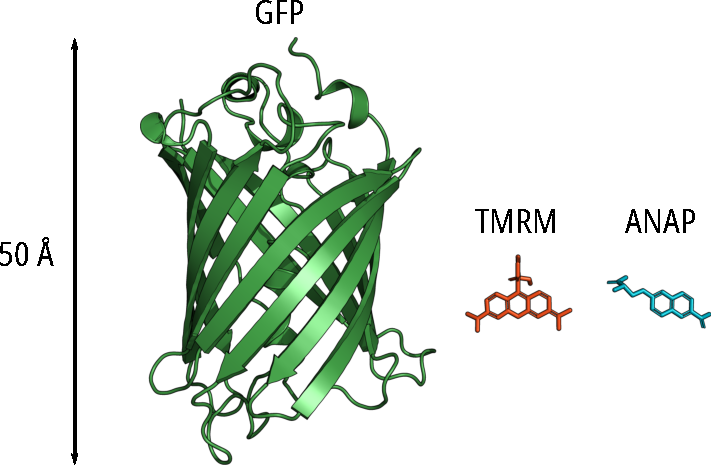
\includegraphics[width=0.7\textwidth]{fluorophore_sizes.pdf}
	\caption[Contrasting sizes of flurophores]{
	{\bf\mccorrect{Contrasting sizes of flurophores.}}
	The molecular structures of three different flurophores used to label proteins; green fluorescent protein (GFP, from PDB \#1GFL), tetramethylrhodamine (TMRM) and L-3-(6-acetylnaphthalen-2-ylamino)-2-aminopropionic acid (ANAP), shown to scale.
	}\label{ch1fig:fluorophore_sizes}
\end{figure}

Finally, ligands and toxins can be fluorescently labelled to investigate the ion channels they regulate \cite{zheng_handbook_2015, braun_current_2020}.
A good illustration of this approach is the use of a fluorescent analogue of cAMP (fcAMP) to study hyperpolarisation-activated cyclic nucleotide-modulated (HCN) pacemaker channels, which are regulated by membrane voltage and the endogenous ligand cAMP.
Binding of fcAMP to HCN channels in membrane patches leads to increased fluorescence at the membrane and activation of channel current, which can be measured simultaneously to correlate ligand binding to channel gating \cite{kusch_interdependence_2010-1, kusch_how_2012, thon_conformational_2015}.
The authors measured the increase in fluorescence and channel current in response to step changes in fcAMP to discriminate between possible models of HCN channel function, and found that their measurements were most consistent with asymmetric contributions of the four subunits of the channel \cite{kusch_how_2012}.
Curiously, conformational states of the channel appeared to be most stable with zero, two or four ligands bound, with the first and third binding steps exhibiting negative cooperativity.

While this series of studies illustrates the power of patch-clamp fluorometry, measuring the fluorescence intensity in membrane patches is not without its pitfalls.
Firstly, the correlation between fluorescence intensity and ligand binding is not perfect.
A necessary assumption is that at saturating fluorescence intensities, the binding sites are fully occupied.
Secondly, careful controls are required to ensure that fluorescence increases are specific to ligand binding to the channel of interest.
\textcite{kusch_interdependence_2010-1} achieved this as described in a previous study \cite{biskup_relating_2007}, by including free fluorescent dye (DY647) in the bath solution, which allowed the authors to separate the specific bound fraction.
Finally, this method is unsuitable for channels with more than one class of binding site for the fluorescent ligand, as it is not possible to assign an increase in fluorescence to ligand binding to one site over another.

\begin{mccorrection}

\section{Summary of objectives}

In the four decades after the first reports of K\ATP{} channel currents in pancreatic \textgreek{b}-cells and their regulation by intracellular adenine nucleotides \cite{ashcroft_glucose_1984-1, rorsman_glucose_1985-1}, there has been a wealth of research attempting to answer a number of fundamental questions, including:
\begin{itemize}
\item How do K\ATP{} channels transduce nucleotide binding at different sites to the channel pore?
\item How do disease-related mutations affect this process?
\item How does SUR1 influence the nucleotide regulation of Kir6.2?
\end{itemize}
Answering these questions definitively has been challenging due to the complex interplay between the different classes of nucleotide binding site, and the difficulty in separating effects on nucleotide binding from effects on transduction and intrinsic channel gating.

In this thesis, I aim to build on previous work and tackle these two challenges, establishing a novel approach to measure nucleotide binding to individual classes of binding site using a combination of electrophysiology and fluorescence techniques.

\end{mccorrection}